\chapter{Domain Decomposition}
\label{chap:domain-decomp}

\newcommand{\lave}{\langle \lambda \rangle}
\newcommand{\lmave}{\langle \overline{\lambda} \rangle}
\newcommand{\dpmax}{\delta{p_i^{max}}}
\newcommand{\pmax}{{p_i^{max}}}
\newcommand{\lmax}{{\lambda_i^{max}}}
\newcommand{\pbar}{\overline{P}}
\newcommand{\lbar}{\overline{\lambda}}

\section{Background}

To this point, we have described methods which will drastically improve
scalability for calculations utilizing thousands or millions of processors. With
these methods, it is possible to effectively utilize leadership class
supercomputers for Monte Carlo calculations --- but there is one caveat. The
simulations would still be forced to rely on parallelism over particles, meaning
that all problem data such as cross sections, tallies, and material compositions
must be replicated on every process. As we began discussing in
\autoref{chap:intro}, data for temperature-dependent cross sections in LWR
simulations may reach upwards of hundreds of gigabytes, and tallies can easily
exceed terabytes of memory. In order to reduce per-node memory requirements, two
strategies have been proposed: domain decomposition and data decomposition. In
this chapter, we will focus on the analysis of domain decomposition for LWR
analysis using Monte Carlo.

In many, if not most, areas of computational physics, spatial domain
decomposition is the most natural and desirable method for achieving
parallelism. Each subdomain is assigned to a different processor, and thus each
processor needs only to work on its subdomain. This makes sense when the work in
the problem is proportional to, and evenly distributed over, the size of the
problem. This is true of most mesh-based methods such as finite difference,
finite element, etc. Monte Carlo particle transport, on the other hand, does not
possess this characteristic. The computational effort in a Monte Carlo
simulation is in transporting the particles; as a result, the work is
unpredictable and not guaranteed to be evenly distributed across a
problem. Moreover, fast-streaming particles can cross the entire problem. Thus,
the use of spatial domain decomposition for Monte Carlo particle transport can
suffer from poor load balancing and overhead from network communication required
for transferring particles between subdomains.

\subsection{Review of Prior Work}

The use of domain decomposition to reduce per-node memory in Monte Carlo
particle transport simulations was first proposed by Alme et al. in 2001
\cite{js-alme-2001}. A slight variation on normal domain decomposition was also
suggested --- instead of just decomposing the geometry, subdomains could also be
replicated. The motivation for this is so that areas of the problem that have a
higher particle density, and hence more work, have proportionally more
processors dedicated to them.

Domain decomposition was subsequently implemented in a production Monte Carlo
code, Mercury, being developed by Lawrence Livermore National Laboratory
\cite{mc-procassini-2007}. A load balancing scheme similar to that proposed by
Alme et al. was also implemented in Mercury whereby the assignment of processors
to domains is periodically adjusted based on the actual work distribution
\cite{mc-procassini-2005}. The initial implementation worked only with
mesh-bashed geometries where the connectivity between regions could be readily
determined. This was later expanded to constructive solid geometries; the
algorithms used for this were described in \cite{mc-greenman-2009}.

Domain decomposition has also been applied to Monte Carlo simulation of thermal
radiation transport \cite{jcp-brunner-2006}. In that work, Brunner et
al. focused on message-passing semantics for domain decomposition schemes,
i.e. how to best communicate particles between processors. This work was later
expanded to include situations where the number of particles in a given
transport sweep was not known \emph{a priori} \cite{jcp-brunner-2009}. However,
in both of those papers, it is explicitly assumed that the problem is perfectly
load balanced, and no solutions are presented for problems that exhibit poor
load balancing.

Finally, domain decomposition is also being implemented in a new Monte Carlo
code, Shift, under development at Oak Ridge National Laboratory
\cite{physor-sly-2012}. The domain decomposition algorithm described by Brunner
\cite{jcp-brunner-2009} was chosen with the added ability to have overlapping
domains to reduce the incidence of particles crossing subdomain boundaries and
hence reduce the overall network communication.

\subsection{Recent Developments}

While the study and application of domain decomposition to Monte Carlo particle
transport simulations now has a ten year history, including the implementation
in two major Monte Carlo codes, there is surprisingly little theoretical
analysis of domain decomposition schemes. In all the papers we've reviewed thus
far \cite{js-alme-2001, mc-procassini-2005, mc-greenman-2009, jcp-brunner-2006,
  jcp-brunner-2009}, arguments about the efficacy of domain decomposition were
made based on measurements in either simple or actual codes. This is good from
the perspective that no assumptions are needed to draw conclusions; however, the
downside is that it is hard to gain an understanding of why or why not domain
decomposition would work in a given problem. In particular, the prior work does
not reveal whether domain decomposed Monte Carlo simulations could be
successfully employed for realistic LWR analysis because the test problems were
not LWR models.

Recognizing the lack of a theoretical foundation with which domain decomposition
algorithms could be analyzed, Siegel et al. published a study in 2012
\cite{jcp-siegel-2012-1} where they attempted to quantify the communication
costs in order to assess the feasibility of carrying out efficient domain
decomposition in a parameter regime relevant to LWR analysis. Key scaling
regimes were identified and performance estimates were carried out over a range
of characteristic parameters. The results demonstrated that for their chosen
model problem, good performance could be attained for reasonable effective
latency and bandwidth values with partition particle densities as low as $10^4$
per node\footnote{The testing platform in \cite{jcp-siegel-2012-1} was the Blue
  Gene/P supercomputer at Argonne National Laboratory.}. This analysis
represents an important step toward quantifying the key theoretical issues and
helped to establish the feasibility of carrying out robust LWR calculations with
Monte Carlo methods.

That being said, the analysis in \cite{jcp-siegel-2012-1} does not address the
impact of initial particle imbalances and small variations in local leakage
rates on evolving particle distributions. If particle communication costs are
potentially manageable in light of typical machine bandwidths and latencies, to
what extent will load imbalances negatively impact performance to the point
where such an approach is no longer a practical alternative? Establishing a
quantitative foundation for this performance penalty will greatly facilitate
weighing tradeoffs in deciding the best path forward among various approaches
for next-generation Monte Carlo codes. In this chapter, this issue is addressed
directly by attempting to quantify the effect of particle load imbalances on the
performance of domain decomposed Monte Carlo algorithms.

In \autoref{sec:domain-decomp-analysis}, an expression for the communication
penalty from load imbalances is derived from theoretical
considerations. However, the starting assumption is that leakage rates are
spatially constant and therefore the expression only accounts for load
imbalances due to the initial particle distribution. In a Monte Carlo
simulation, the stochastic nature of the solution will result in spatially
varying leakage rates. This is explicitly accounted for in
\autoref{sec:variable-leakage}; the resulting expression appears similar to that
derived in \autoref{sec:domain-decomp-analysis} but with an extra factor
accounting for the variable leakage rates. Finally, in
\autoref{sec:domain-decomp-evaluation}, measured data from simulations of the
Monte Carlo performance benchmark using OpenMC are used to evaluate the load
imbalance penalty for various domain sizes.

The analysis and results from this chapter are derived from a paper accepted for
publication in \emph{Journal of Computational Physics} \cite{jcp-siegel-2012-2}.

\section{Analysis}
\label{sec:domain-decomp-analysis}

\subsection{Problem definition}

To fully define the problem, let us begin with a domain $X$ segmented into $N$
non-overlapping partitions $X = \cup x_j, j=1,\dotsc,N$. In a light-water
reactor, these partitions might be chosen for convenience to be a full fuel
assembly or some part of an assembly. If we denote the initial number of
particles on partition $x_j$ as $p_{0,j}$, then the initial global particle
count $P_0$ is given by:
\begin{equation}
  \label{eq:globalP}
  P_0 = \sum_{j=1}^{N} p_{0,j}.
\end{equation}
For simplicity, assume that each partition is mapped to a single process in a
three-dimensional virtual Cartesian topology of $N$ processes. As in
\autoref{chap:fission-bank}, we are assuming a one-to-one mapping of processes
to processors, and thus we use the terms \emph{processor}, \emph{partition}, and
\emph{process} interchangeably.

On a given partition, particles local to that partition are advanced through a
sequence of interactions until they are either 1) absorbed\footnote{In a
  non-analog simulation, particles can also be killed from Russian roulette or
  other variance reduction techniques.} or 2) reach a processor boundary. For
optimal performance particles that reach the boundary are buffered locally until
all particle trajectories are computed, and are subsequently exchanged with
neighboring processors. We refer to the particle exchange phase of this process
as a \emph{stage}, and to a complete set of stages (i.e. until all particles are
absorbed) as a \emph{generation}. At the end of each generation, the fission
source is updated and the next generation begins.

Define the particle \textit{local leakage} $\lambda$ on each $x_j$ for a given
stage $i$ as
\begin{equation*}
  \lambda_{i,j} = \frac{\mbox{number of particles leaving $x_j$ at stage
      $i$}}{\mbox{number of particles starting in $x_j$ at stage $i$}}.
\end{equation*}
The goal of this analysis is to estimate the impact of initial particle load
imbalances and spatially varying local leakage values on previous performance
estimates of domain-decomposed LWR simulations.  We refer to the perfectly load
balanced, constant leakage scenario as the \emph{ideal} case. This was explored
in depth in \cite{jcp-siegel-2012-1}, where it was shown that communication
costs imposed a reasonable penalty on overall simulation time for a broad range
of relevant parameter values.

Following \cite{scott-2005} we first define the \emph{load balance} $\Gamma_i$
at each stage $i$ as
\begin{equation}
  \Gamma_i = \frac {\overline{P}_i}{p_i^{max}},
\end{equation}
where
\begin{equation*}
  \overline{P}_i = \frac{1}{N}\sum_{j=1}^{N} p_{i,j}
\end{equation*}
and $p_i^{max}$ denotes the maximum particle count on a partition at stage $i$.
The amount the load balance $\Gamma_i$ differs from the ideal case $\Gamma = 1$
measures the relative difference between the highest particle and average
particle counts:
\begin{equation}
  1- \Gamma_i = \frac{p_i^{max} - \overline{P}_i}{p_i^{max}}.
\end{equation}
Note that unlike \cite{scott-2005} we express the load imbalance in terms of
particle densities rather than execution time. Their equivalence will be argued
in the following section.

We seek to estimate a related but distinct quantity --- an upper bound for the
relative difference between the total simulation time per generation of the
non-ideal case and the ideal case. We define this relative difference as the
\textit{load imbalance penalty} $\Delta$:
\begin{equation}
  \label{eq:load-imbalance}
  \Delta = \frac{\tau' - \tau}{\tau} = \frac{\tau'}{\tau} - 1,
\end{equation}
where $\tau$ denotes the total simulation time per generation in the ideal case,
and $\tau'$ for the non-ideal case.  Note that an expression for $\Delta$ must
include both the particle tracking as well as the communication costs across all
stages of a given generation. While related to the per-stage particle load
balance, the load imbalance penalty is a distinct quantity.

\subsection{Basic properties}

Given this simple problem definition above, it is clear that, for purely
reflective boundary conditions (a good approximation for reflectors in power
reactors) the \emph{global} number of particles at any \emph{stage} is given by
\begin{equation}
  \label{eq:pg}
  P_{i+1} = \sum_{j=1}^N p_{i+1,j} = \sum_{j=1}^N \lambda_{i,j}
  p_{i,j} \hspace{.5in} i=0,1,\dotsc,M-1
\end{equation}
where $M$ denotes the final stage in the generation --- i.e. when all particles
are absorbed and none remain. We emphasize again that $P_i$ denotes the global
particle count at stage $i$ while $p_{i,j}$ denotes the local particle count on
partition $j$ at stage $i$.

To estimate $\tau'$, the per-generation simulation time in the non-ideal case,
we seek an expression for the \emph{local} particle distribution --- i.e. the
number of particles on each partition $x_j$ at stage $i$. Assuming isotropic
leakage, the neutron count on a partition is given by:
\begin{equation}
  \label{eq:pl}
  p_{i+1,j} = \frac{1}{6} \left( \lambda_{i,j1}p_{i,j1} + \lambda_{i,j2}p_{i,j2}
  + \dotsb + \lambda_{i,j6}p_{i,j6} \right)
\end{equation}
where $j1,j2,\dotsc,j6$ denote the six immediate neighbors of partition $j$ on a
Cartesian lattice. Equation \eqref{eq:pl} simply states that, in advancing
stages, a given partition receives 1/6th of the leaked particles from each of
its six neighbors on a Cartesian grid.

Equation \eqref{eq:pl} shows that the evolution of the local particle
distributions depends on the detailed alignment of the local particle counts and
the local leakage rates. To reduce it further requires additional
assumptions. We start by noting that, in an LWR, the neutron spectrum and
material heterogeneities are roughly constant from partition to partition (this
property is demonstrated using simulation data in
\autoref{sec:domain-decomp-evaluation}). This observation makes the case of
approximately spatially uniform local leakages of great practical interest in
the present context, and thus we initially consider the case of $\lambda_{i,j} =
\lambda_i$. Note that we still expect non-trivial per-stage variation in
leakages as neutron energies will shift toward the thermal range with increasing
stages. Important model corrections for small spatial variations in $\lambda$
will be considered in \autoref{sec:variable-leakage}.

For spatially constant $\lambda$, \eqref{eq:pg} then becomes
\begin{align}
  \label{eq:pg2}
  P_{i} &= \sum_{j=1}^N \lambda_{i-1} p_{i-1,j} = \lambda_{i-1}
  \sum_{j=1}^Np_{i-1,j} = \lambda_{i-1} P_{i-1} \nonumber \\
  &= \lambda_{i-1} \lambda_{i-2} \dotsm \lambda_{0} P_0 \nonumber \\
  &\approx {\lave}^{i} P_0 \hspace{2in} i=1,2,\dotsc,M
\end{align}
where $\lave$ is defined as the geometric mean of the leakage rate,
\begin{equation}
  \label{eq:cycle_mean}
  \lave = \sqrt[M]{\lambda_{M-1}\lambda_{M-2} \dotsm \lambda_{0} }.
\end{equation}
Equation \eqref{eq:pl} then simplifies to
\begin{equation}
  \label{eq:meanp}
  p_{i+i,j} = \frac{\lambda_i}{6} \left( p_{i,j1} + p_{i,j2} + \cdots + p_{i,j6}
  \right)
\end{equation}
Equation \eqref{eq:meanp} shows that, for spatially constant $\lambda$, at each
subsequent stage each partition has the average value of the total leaked
particles from the neighboring partitions in the previous stage.  Equation
\eqref{eq:pg2} shows that, in the case of constant $\lambda$, the particle load
imbalance does not affect the number of stages required to complete a
generation, which can be estimated by setting $P_i = 1$ in \eqref{eq:pg2}:
\begin{equation}
  \label{eq:kfinal}
  {\lave}^M P_0 = 1 \implies M \approx -\frac{\log P_0}{\log \lave}.
\end{equation}
Both properties are used in the analysis that follows.

\subsection{Expression for \texorpdfstring{$\tau$}{tau}}

Given these basic properties, we first seek an estimate of the total
per-generation cost in the idealized case of an initial even distribution of
particles and spatially constant $\lambda$.  This is accomplished by decomposing
$\tau$ into a local work $\tau_l$ and inter-process communication $\tau_c$
component as
\begin{equation}
  \tau = \tau_l + \tau_c.
\end{equation}
In the case of perfect load balancing and assuming a roughly equal distribution
of track length and neutron spectra across partitions (i.e. our earlier
assumption of constant $\lambda$), the local work $\tau_l$ should be roughly
proportional to the total number of particles tracked on a partition in a given
generation,
\begin{equation}
  \label{eq:loc_work}
  \tau_{l} \approx \mu \sum_{i=0}^{M} \overline{P}_{i},
\end{equation}
where the constant $\mu$ is a measure of the tracking time per particle, and
where it is understood that the particle count $p_{i,j}$ is the same on any
given partition, since all partitions are equivalent in the ideal case.

The communication time $\tau_c$ can be further decomposed into a latency and
bandwidth component \cite{jcp-siegel-2012-1}. For each generation, a total of
$M$ messages need to be sent to each processor's six neighbors, so in general
the total time per generation due to message latency can be modeled as
proportional to $6 \alpha M$, where $\alpha$ is some measure of the effective
application-level latency for a single send.

If we ignore the dependence of $\lambda$ on stage, by definition $\lambda
\overline{P}_i$ particles are sent from each processor at stage $i$, and the
total number of particles sent in a generation from any processor is $\lambda
\sum_i \overline{P}_i$. Thus, the bandwidth term can be roughly modeled as
$\beta \lambda \sum_i \overline{P}_i$, where $\beta$ denotes the effective
inverse bandwidth for nearest-neighbor exchanges (expressed in time per
particle).

When we account for stage dependence $\lambda$ is replaced by $||\lambda||$,
defined as the solution to the $M$th order polynomial:
\begin{equation}
  \label{eq:lmean}
  \sum_{i=1}^M ||\lambda||^i = \lambda_0 + \lambda_1\lambda_0 + \cdots +
  \lambda_{M-1}\lambda_{M-2}\dotsm\lambda_0.
\end{equation}
The bandwidth term can then be written as:
\begin{align}
  \beta \sum_{i=0}^{M-1} \lambda_i \overline{P}_i &= \beta(\lambda_0
  \overline{P}_0 + \lambda_1 \overline{P}_1 + \dotsb +
  \lambda_{M-1}\overline{P}_{M-1}) \nonumber \\
  &= \beta(\lambda_0 \pbar_0 + \lambda_1 \lambda_0 \pbar_0 + \dotsb +
  \lambda_{M-1}\lambda_{M-2}\dotsm\lambda_0 \pbar_0) \nonumber \\
  &=\beta\pbar_0(\lambda_0 + \lambda_1\lambda_0 + \dotsb +
  \lambda_{M-1}\lambda_{M-2}\dotsm\lambda_0) \nonumber \\
  &= \beta\pbar_0\sum_{i=1}^M ||\lambda||^i.
\end{align}
Using these relations together with \eqref{eq:kfinal} then yields the following
expression for the total communication time:
\begin{equation}
  \label{eq:tot_comm}
  \tau_c = -6 \alpha \frac{\log P_0}{\log \lave} + \beta\pbar_0\sum_{i=1}^M
  ||\lambda||^i.
\end{equation}
Using the same approach on \eqref{eq:loc_work} and combining with
\eqref{eq:tot_comm} gives the final expression for total simulation time in the
idealized case:
\begin{align}
  \label{eq:tau1}
  \tau &= -6 \alpha \frac{\log P_0}{\log \lave} + \mu \pbar_0 \sum_{i=0}^M
  ||\lambda||^i + \beta\pbar_0\sum_{i=1}^M ||\lambda||^i \nonumber \\
  &= -6 \alpha \frac{\log P_0}{\log \lave} + \left ( \mu \sum_{i=0}^M
  ||\lambda||^i + \beta\sum_{i=1}^M ||\lambda||^i \right ) \pbar_0.
\end{align}

\subsection{Expression for \texorpdfstring{$\tau'$}{tau'}}

We now seek an estimate for the total simulation time $\tau'$ in the presence of
an initial load imbalance. For convenience we first express $p_{i,j}$ as a
combination of partition mean and fluctuating parts. That is,
\begin{equation}
  \label{eq:mean}
  \delta p_{i,j} = p_{i,j} - \overline{P}_i.
\end{equation}
When a load imbalance is present the partition with the largest particle count
controls the total performance cost. If we denote the particle count on this
process as $p^{max}_i = \overline{P}_i + \dpmax$, then by the same logic as in
the previous section, the load-imbalanced performance is:
\begin{equation}
  \label{eq:tauprime-1}
  \tau' = -6 \alpha \frac{\log P_0}{\log \lave} + \mu \sum_{i=0}^M p_i^{max} +
  \beta \sum_{i=0}^{M-1} \lambda_i p_i^{max}.
\end{equation}
While we cannot directly evaluate the sum of $p_i^{max}$, a simple upper bound
can be derived by recognizing that, assuming roughly equal leakage to each
neighbor, the largest possible value of $p$ at stage $i+1$ occurs if all six
neighbors of a partition contain $p_i^{max}$ particles. Thus,
\begin{equation}
  \label{eq:pmax-ub1}
  p^{max}_{i+1} \le \lambda_i p^{max}_i.
\end{equation}
This implies that
\begin{align}
  \label{eq:pmax-expand1}
  \sum_{i=0}^M p_i^{max} &\le \mu \left ( p_0^{max} + \lambda_0 p_0^{max} +
  \lambda_1 \lambda_0 p_0^{max} + \dotsb + \lambda_{M-1} \lambda_{M-2} \dotsm
  \lambda_0 p_0^{max} \right ) \nonumber \\
  &= \mu p_0^{max} \left ( 1 + \lambda_0 + \lambda_1 \lambda_0 + \dotsb +
  \lambda_{M-1} \lambda_{M-2} \dotsm \lambda_0 \right ) \nonumber \\
  &= \mu p_0^{max} \sum_{i=0}^M ||\lambda||^i
\end{align}
and
\begin{align}
  \label{eq:pmax-expand2}
  \sum_{i=0}^{M-1} \lambda_i p_i^{max} &\le \mu \left ( \lambda_0 p_0^{max} +
  \lambda_1 p_1^{max} + \dotsb + \lambda_{M-1} p_{M-1}^{max} \right ) \nonumber \\
  &= \mu \left ( \lambda_0 p_0^{max} + \lambda_1 \lambda_0 p_0^{max} + \dotsb +
  \lambda_{M-1} \lambda_{M-2} \dotsm \lambda_0 p_0^{max} \right ) \nonumber \\
  &= \mu p_0^{max} \left ( \lambda_0 + \lambda_1 \lambda_0 + \dotsb +
  \lambda_{M-1} \lambda_{M-2} \dotsm \lambda_0 \right ) \nonumber \\
  &= \mu p_0^{max} \sum_{i=1}^M ||\lambda||^i.
\end{align}
Substituting \eqref{eq:pmax-expand1} and \eqref{eq:pmax-expand2} into
\eqref{eq:tauprime-1}, we obtain
\begin{align}
  \label{eq:tauprime-2}
  \tau' &= -6 \alpha \frac{\log P_0}{\log \lave} + \mu p_0^{max} \sum_{i=0}^M
  ||\lambda||^i + \beta p_0^{max} \sum_{i=1}^M ||\lambda||^i \nonumber \\
  &= -6 \alpha \frac{\log P_0}{\log \lave} + \left( \mu \sum_{i=0}^M
  ||\lambda||^i + \beta \sum_{i=1}^M ||\lambda||^i \right ) p_0^{max}.
\end{align}
With expressions for $\tau$ and $\tau'$, we can now proceed to estimate the load
imbalance penalty.

\subsection{Expression for \texorpdfstring{$\Delta$}{Delta}}

Using \eqref{eq:load-imbalance}, \eqref{eq:tau1}, and \eqref{eq:tauprime-2} and
noting that $p_0^{max} = \pbar_0 + \delta p_0^{max}$, we get the following
expression for $\Delta$:
\begin{equation}
  \label{eq:delta1}
  \Delta = \frac{\displaystyle \left( \mu \sum_{i=0}^M ||\lambda||^i + \beta
    \sum_{i=1}^M ||\lambda||^i \right ) \delta p_0^{max}}{\displaystyle -6
    \alpha \frac{\log P_0}{\log \lave} + \left ( \mu \sum_{i=0}^M ||\lambda||^i
    + \beta\sum_{i=1}^M ||\lambda||^i \right ) \pbar_0}.
\end{equation}
We can simplify \eqref{eq:delta1} slightly by dividing each term by the
expression in parentheses, i.e.
\begin{equation}
  \label{eq:delta2}
  \Delta = \frac{\delta p_0^{max}}{\displaystyle -6 \alpha \frac{\log P_0}{\log
        \lave} \left( \mu \sum_{i=0}^M ||\lambda||^i + \beta \sum_{i=1}^M
      ||\lambda||^i \right )^{-1} + \pbar_0}.
\end{equation}
The first term in the denominator of \eqref{eq:delta2} measures the importance
of latency relative to bandwidth and tracking timescales, which is presumed to
be small for typical problem sizes and parameter regimes (e.g. see
\cite{jcp-siegel-2012-1}) but which is retained here for the sake of generality.
Note that \eqref{eq:delta2} implies that
\begin{equation}
  \label{eq:delta3}
  \Delta \le \frac{\delta p_0^{max}}{\overline{P_0}} = \frac{1}{\Gamma_0} - 1,
\end{equation}
which should be a good approximation for applications where the latency term is
much smaller than the bandwidth and tracking terms. We see, then, that assuming
spatially constant $\lambda$ and given isotropic neutron local leakage and
constant mean tracking rates per partition, we can establish an upper bound for
$\Delta$ entirely in terms of the initial particle configuration.

\section{Variable leakage rates}
\label{sec:variable-leakage}

Equation \eqref{eq:delta2} should give a reasonable estimate for reactor
applications across a range of parameter values, where material inhomogeneities
are roughly equally distributed and thus local leakage rates show very little
variation. However, it fails to capture a critical effect that emerges as we
move to smaller partition sizes, and which sets an important limit on the
utility of the domain-decomposed approach. To see this we explicitly account for
spatially variant, non-constant leakage in the formulation of the model.

Consider a distribution of leakage rates across partitions at a given stage with
a maximum value defined as:
\begin{equation}
  \lambda^{max}_i = \max \left\{\lambda_{i,j} : 1 \le j \le N\right\}.
\end{equation}
In estimating the computation time for this scenario compared to the ideal case
(i.e. calculating $\Delta$), the question arises of what corresponding spatially
constant value of $\lambda$ should be used for the ideal case. Several options
are reasonable, but here we choose a mean value that preserves
stages. Specifically, if we define a particle-weighted mean leakage as:
\begin{equation}
  \label{eq:pmean}
  \lbar_i = \frac{\sum_{j=1}^{N} p_{i,j} \lambda_{i,j}}{P_i}
\end{equation}
then the ideal and non-ideal cases are guaranteed to have the same number of
global particles at successive stages:
\begin{equation*}
  \frac{P_{i+1}}{P_i} = \frac{1}{P_i}\sum_{j=1}^N \lambda_{i,j} p_{i,j} =
  \lbar_i.
\end{equation*}
Thus, the performance for the ideal case with variable leakage rates is now
\begin{align}
  \label{eq:tau2}
  \tau &= -6 \alpha \frac{\log P_0}{\log \lmave} + \mu \sum_{i=0}^M
  \overline{P}_i + \beta \sum_{i=0}^{M-1} \lbar_i \overline{P}_i
  \nonumber \\ &= -6 \alpha \frac{\log P_0}{\log \lmave} + \left ( \mu
  \sum_{i=0}^M ||\lbar||^i + \beta\sum_{i=1}^M
  ||\lbar||^i \right ) \pbar_0
\end{align}
where $\lmave$ is the geometric mean (over stages) of the particle-weighted mean
leakage at each stage, i.e.
\begin{equation*}
    \lmave = \sqrt[M]{\lbar_{M-1}\lbar_{M-2} \dotsm
      \lbar_{0}}.
\end{equation*}
and $||\lbar||$ is defined analogous to \eqref{eq:lmean}:
\begin{equation*}
  \sum_{i=1}^M ||\lbar||^i = \lbar_0 + \lbar_1 \lbar_0 + \dotsb + \lbar_{M-1}
  \lbar_{M-2} \dotsm \lbar_0.
\end{equation*}
Following \eqref{eq:pmax-ub1}, then, the largest possible particle count at
stage $i$ occurs on partition $x_j$ if on its six neighbors $\pmax$ coincides
with $\lmax$. That is,
\begin{equation}
  \label{eq:ub2}
  p_{i+1}^{max} \le \lmax p_i^{max}.
\end{equation}
This implies that
\begin{equation}
  \tau' \le -6\alpha\frac{\log P_0}{\log \lmave} + \mu \sum_{i=0}^M \pmax
  \nonumber + \beta \sum_{i=0}^{M} \lmax \pmax.
\end{equation}
Following the same logic as in \eqref{eq:pmax-expand1}, \eqref{eq:pmax-expand2},
and \eqref{eq:tauprime-2} we can derive an upper bound for $\tau'$ in the case
of variable $\lambda$:
\begin{equation}
  \label{eq:tauprime-3}
  \tau' \le -6 \alpha \frac{\log P_0}{\log \lmave} + \left( \mu \sum_{i=0}^M
  ||\lambda^{max}||^i + \beta \sum_{i=1}^M ||\lambda^{max}||^i \right )
  p_0^{max}
\end{equation}
where $||\lambda^{max}||$ is defined as
\begin{equation*}
  \sum_{i=1}^M ||\lambda^{max}||^i = \lambda^{max}_0 + \lambda^{max}_1
  \lambda^{max}_0 + \dotsb + \lambda^{max}_{M-1} \lambda^{max}_{M-2} \dotsm
  \lambda^{max}_0.
\end{equation*}
We can then use \eqref{eq:tau2} and \eqref{eq:tauprime-3} to obtain the
following upper bound for the load imbalance:
\begin{equation}
  \label{eq:delta4}
  \Delta \le \frac{\displaystyle -6 \alpha \frac{\log P_0}{\log \lmave} + \left(
    \mu \sum_{i=0}^M ||\lambda^{max}||^i + \beta \sum_{i=1}^M
    ||\lambda^{max}||^i \right ) p_0^{max}}{\displaystyle -6 \alpha \frac{\log
      P_0}{\log \lmave} + \left ( \mu \sum_{i=0}^M ||\lbar||^i +
    \beta\sum_{i=1}^M ||\lbar||^i \right ) \pbar_0} - 1.
\end{equation}
Again, taking the very reasonable assumption (see e.g. \cite{jcp-siegel-2012-1})
that the latency term is small relative to the sum of the bandwidth and tracking
terms, we can establish a more intuitive upper bound:
\begin{equation}
  \label{eq:delta5}
  \Delta \le \frac{C}{\Gamma_0} - 1.
\end{equation}
where we have defined the factor $C$ as
\begin{equation}
  \label{eq:correction1}
  C = \frac{\displaystyle \mu \sum_{i=0}^M ||\lambda^{max}||^i + \beta
    \sum_{i=1}^M ||\lambda^{max}||^i}{\displaystyle \mu \sum_{i=0}^M ||\lbar||^i
    + \beta\sum_{i=1}^M ||\lbar||^i}.
\end{equation}
One can interpret this as follows --- accounting for variable leakage rates has
introduced a ``correction factor'' relative to \eqref{eq:delta3}; clearly, when
$||\lbar|| = ||\lambda^{max}||$, \eqref{eq:delta5} reduces to
\eqref{eq:delta3}. Further simplification can be made to \eqref{eq:correction1}
by writing
\begin{equation}
  \label{eq:correction2}
  C = \frac{\displaystyle \mu + \beta \frac{\sum_{i=1}^M
      ||\lambda^{max}||^i}{\sum_{i=0}^M ||\lambda^{max}||^i}}{\displaystyle \mu
    + \beta \frac{\sum_{i=1}^M ||\lbar||^i}{\sum_{i=0}^M ||\lbar||^i}}
  \frac{\sum_{i=0}^M ||\lambda^{max}||^i}{\sum_{i=0}^M ||\lbar||^i}
\end{equation}
and subsequently using the approximation
\begin{equation}
  \label{eq:sum-approx}
  \sum_{i=1}^M x^i \approx x \sum_{i=0}^M x_i
\end{equation}
which should hold for $M$ large. Applying \eqref{eq:sum-approx} to
$||\lambda^{max}||$ and $||\lbar||$ in \eqref{eq:correction2} yields
\begin{equation}
  \label{eq:correction3}
  C \approx \frac{\mu + \beta ||\lambda^{max}||}{\mu + \beta ||\lbar||}
  \frac{\sum_{i=0}^M ||\lambda^{max}||^i}{\sum_{i=0}^M ||\lbar||^i}.
\end{equation}
The greater the spatial variation in leakage rates the more the system bandwidth
and neutron tracking rates factor into the performance. The implications of
these formulas are explained in the simple tests below, where we aim to estimate
$C$ as a function of the main problem parameters.

\section{Evaluation of model}
\label{sec:domain-decomp-evaluation}

For a given initial particle configuration, evaluation of the model equation
\eqref{eq:delta4} requires estimates for the particle tracking rate $\mu$, the
application-level inverse bandwidth $\beta$ and latency $\alpha$, and the local
leakage rate estimates from which to compute $||\lambda^{max}||$ and
$||\lbar||$. These parameters vary widely by both machine and specific code
application. Here we evaluate these terms in a parameter regime relevant to LWR
physics on modern supercomputers. Other applications and machine architectures
can be evaluated with appropriate values of these parameters.

\subsection{Leakage rates}

While best-estimate application-level bandwidth and latency terms can be
estimated from standard benchmarks (e.g. \cite{cpe-wallcraft-2000}), the leakage
rate terms in \eqref{eq:delta4} are more difficult to approximate. Simplified
models, such as the Wigner rational approximation \cite{ae-pashkin-1970} provide
rough estimates of expected domain-dependent leakage rates, but do a poor job at
estimating stage dependence. Thus, to be as precise as possible we measure these
values directly using an existing Monte Carlo particle transport code --- OpenMC
\cite{ane-romano-2013}. Note that, though parallel, OpenMC does not employ
domain decomposition. To model partitions and stages, we overlay within OpenMC
an imaginary grid decomposition and effectively measure the behavior of
particles between fictional stages during a generation. The resulting particle
loads and number of stages should be identical to a truly domain decomposed code
using an identical computational grid.

The specific test executed was based on the Monte Carlo Performance benchmark
\cite{mc-hoogenboom-2011} using $0.5$ billion active particle histories.
Leakage rates at each stage and within each partition were measured for three
cases: a single assembly, quarter-assembly, and ninth-assembly partition overlay
using 20, 40, and 60 axial levels, respectively. In each case, the benchmark
model was simulated on a 19-node Intel Xeon dual core cluster with 1 million
neutrons per generation for 150 inactive and 500 active generations. For neutron
cross-sections, data from ENDF/B-VII.0 was used.

\autoref{fig:leakage-maps} illustrates the scale and level of variation in local
leakage rates for the full, quarter, and one-ninth assembly cases.  The plots
shown are for the axial level nearest the middle of the core at stage zero. They
represent ``typical'' leakage rate distributions and are intended to graphically
illustrate their relative lack of spatial coherency and small range of
values. Also, it is evident from the figure that, as expected, leakage rates
increase non-trivially with decreasing partition size.
\begin{figure}[ht!]
  \centering
  \includegraphics[width=2.5in]{figures/ch5/leakage_map1.png}
  \includegraphics[width=2.5in]{figures/ch5/leakage_map1_4.png}
  \includegraphics[width=2.5in]{figures/ch5/leakage_map1_9.png}
  \caption{Leakage rate distributions for the full, quarter, and ninth assembly
    experiments.}
  \label{fig:leakage-maps}
\end{figure}
To see this more clearly, \autoref{fig:avg-leakage} shows the stage-dependent
mean and standard deviation (error bar overlay) of $\lambda$ for each
simulation.  In each case, we see the clear trend that as neutrons thermalize
(undergo successive collisions), the leakage rates decrease corresponding to a
shorter mean free path. Furthermore, the superposed standard deviations indicate
extremely small spatial variation in the first several stages, which accounts
for the majority of data movement and performance cost. When particle counts are
small in later stages statistical variations result in larger standard deviation
values, but their impact on total performance is expected to be small. We note
that this very small spatial variation hints that the correction factor for
variable $\lambda$ in \eqref{eq:correction1} may be small. This is evaluated in
the next section.
\begin{figure}[ht!]
  \centering
  \includegraphics[width=4.0in]{figures/ch5/avg_leakage.pdf}
  \caption{Average values of leakage rate $\lambda$ at each stage for the full,
    quarter, and ninth assembly experiments.}
  \label{fig:avg-leakage}
\end{figure}

We next test the predictions for total number of stages $M$ per generation given
by \eqref{eq:kfinal}, i.e.
\begin{equation}
  \label{eq:totalstages}
  M = -\frac{\log P_0}{\log \lmave}.
\end{equation}
The values of the $\lmave$ were calculated for each of the three experiments and
plugged into the \eqref{eq:totalstages}. \autoref{tab:num-stages} compares these
results with those obtained directly from the simulation. The model formula
behaves as expected, differing by only several percent from the measured
data. Exact correspondence is not expected --- statistical fluctuations, slight
anisotropies and other minor effects are likely to yield small variations. For
practical purposes though the current estimate is more than adequate.
\begin{table}[htb]
  \centering
  \begin{tabular}{c c c}
    \toprule
    Experiment & $M$ (data) & $M$ (model)  \\
    \midrule
    Full assembly & $41$ & $39$  \\
    Quarter assembly & $52$ & $51$ \\
    Ninth assembly & $71$ & $70$  \\
    \bottomrule
  \end{tabular}
  \caption{The number of stages $M$ for the three numerical experiments vs. the
    value predicted by \eqref{eq:totalstages}.}
  \label{tab:num-stages}
\end{table}

It is furthermore instructive to test the fidelity of \eqref{eq:ub2} to the true
measure maximum particle counts at each stage. While \eqref{eq:ub2} is a true
statement, in a practical sense it is of questionable value if it over-predicts
$p^{max}_i$ by too significant a margin. \autoref{fig:ub-source} shows the
computed value of $p^{max}_i$ for each stage versus the value predicted by
\eqref{eq:ub2}. Given that leakage rate variation is very small spatially, it is
not surprising to see that \eqref{eq:ub2} works extremely well as an upper
bound, over-predicting the measured value by less than $1.0\%$ for the initial
stages (which account for the bulk of the particle transfers).
\begin{figure}[ht!]
  \centering
  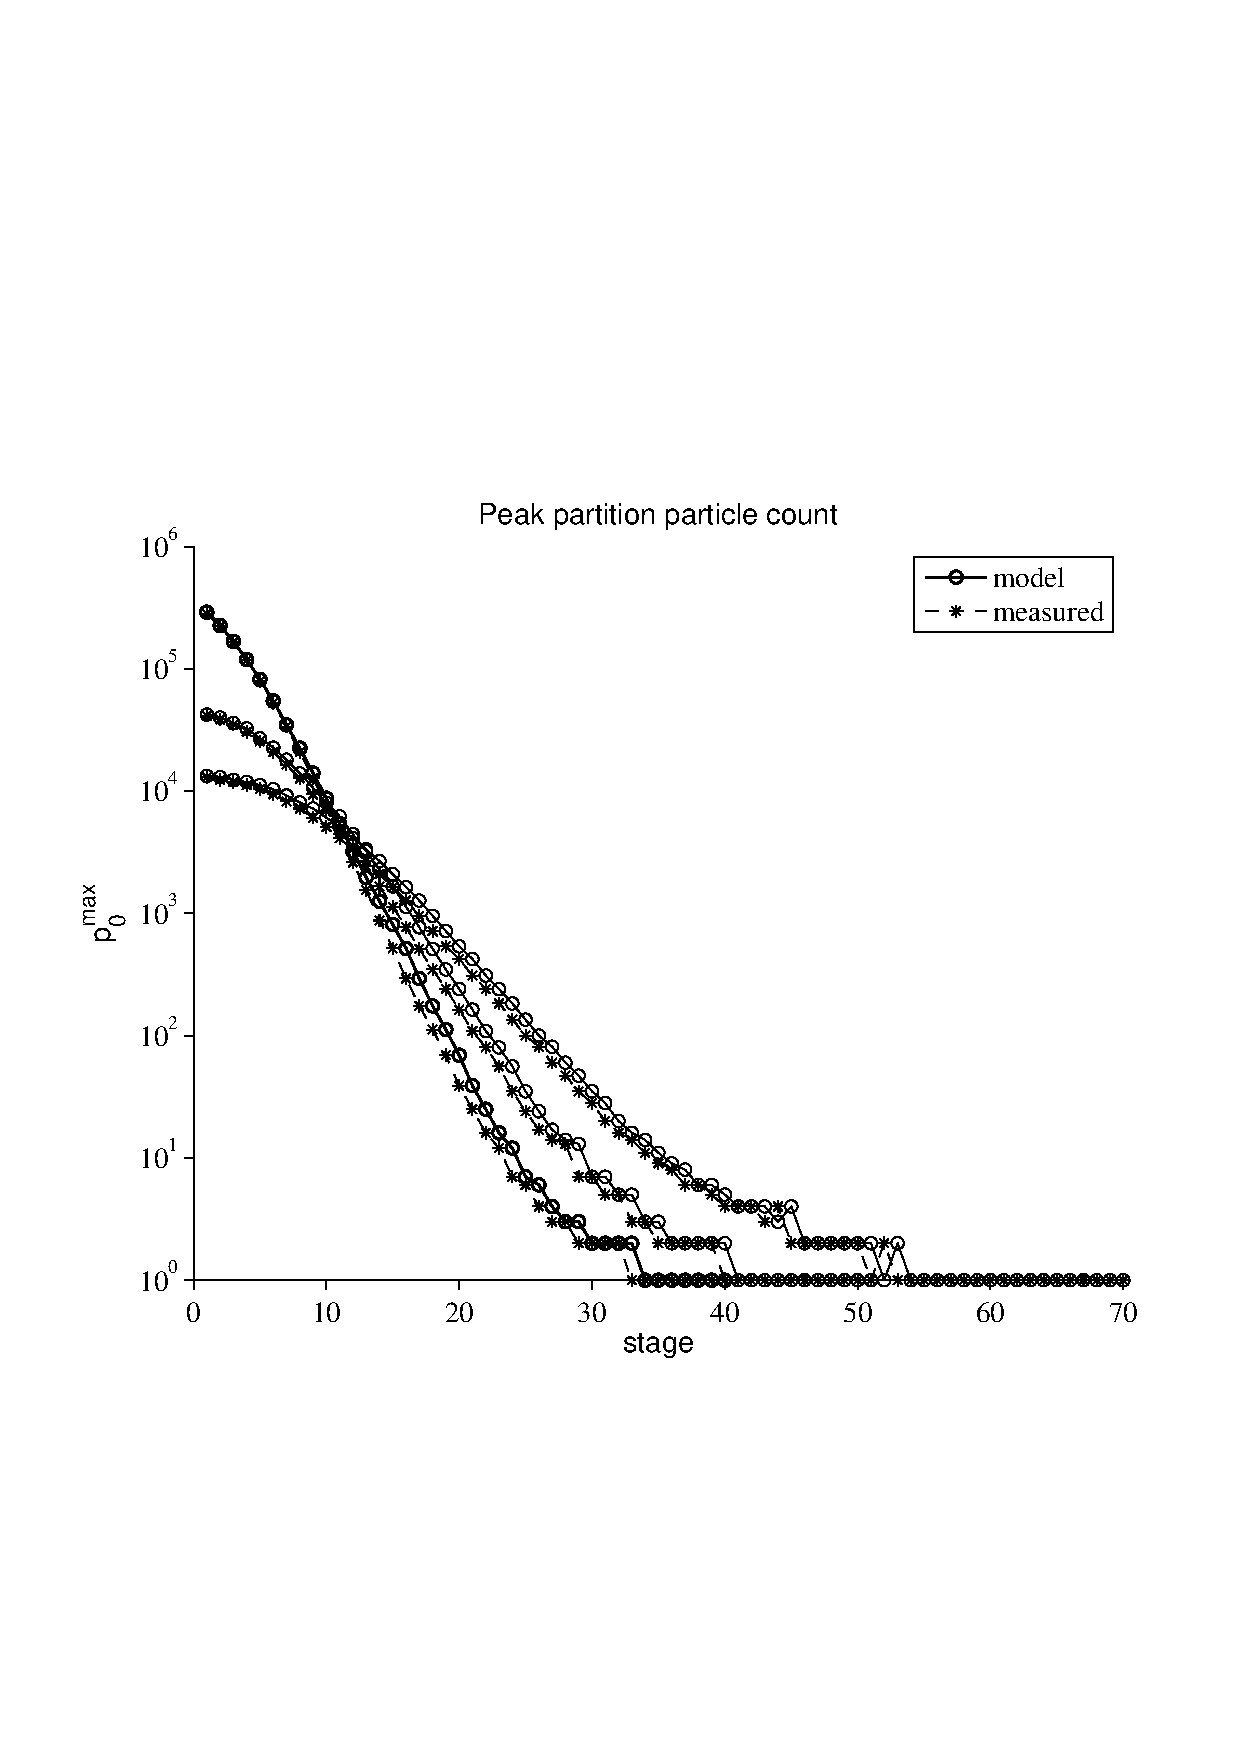
\includegraphics[width=4.0in]{figures/ch5/ub_source.pdf}
  \caption{Computed values of $p^{max}$ for each stage versus the value
    predicted by \eqref{eq:ub2}.}
  \label{fig:ub-source}
\end{figure}

\subsection{Evaluation of correction factor $C$ and penalty \texorpdfstring{$\Delta$}{Delta}}

Given an initial particle configuration and reasonable estimates for leakage, it
remains to evaluate $C$ in \eqref{eq:correction1}. To reiterate, under the
assumption of spatially constant leakage $C$ is unity and the load imbalance
penalty can be upper bounded by the initial particle configuration as
$\frac{p_0^{max}}{\overline{P_0}}$. When leakage rates vary spatially $C$
measures the amplification of the performance penalty. We estimate $C$ in two
steps, first evaluating the contribution of the bandwidth and tracking times,
given by the first term in \eqref{eq:correction3}:
\begin{equation}
  \label{eq:C-factor-ratio}
  \frac{\mu + \beta ||\lambda^{max}||}{\mu + \beta ||\lbar||} = \frac{1 +
    \frac{\beta}{\mu}||\lambda^{max}||}{1 + \frac{\beta}{\mu}||\lbar||}.
\end{equation}
Note that for any conventional machine $\beta \ll \mu$, reflecting that tracking
rates are much slower than inter-processor communication, and since $||\lbar||
\sim ||\lambda^{max}||$, \eqref{eq:C-factor-ratio} remains very close to unity
and contributes negligibly to the overall load imbalance. This demonstrates the
important fact that for all practical purposes the system bandwidth and latency
have very little effect on the load imbalance penalty, which is determined
almost entirely by the physics of neutron transport as expressed by the local
leakage rates.

The second contribution of $C$ is the second term in \eqref{eq:correction3}:
\begin{equation*}
  \frac{\sum_{i=0}^M ||{\lambda^{max}}||^i}{\sum_{i=0}^M
    ||\lbar||^i}.
\end{equation*}
Note that unlike \eqref{eq:C-factor-ratio} this term becomes problematic as the
processor grid is refined, since we intuitively expect maximum leakage rates of
unity for sufficiently small domains. Assuming that this is the case, the
numerator is upper bounded by $1+M$. If the average value does not approach
unity, the Taylor series approximation should be a good approximation and we can
rewrite this expression as:
\begin{equation*}
  \frac{\sum_{i=0}^M ||{\lambda^{max}}||^i}{\sum_{i=0}^M
    ||\lbar||^i} \le (1+M)(1-||\lbar||).
\end{equation*}
While this term is likely a modest fraction of the total number of stages, we
must recall that $M$, the number of stages itself, increases rapidly with
decreasing partition size, and even a small fraction could easily significantly
amplify the load imbalance.

To explore this in greater depth requires use of the OpenMC simulation
results. \autoref{tab:delta} shows the results, including the model predictions
for the load imbalance penalty for the full, quarter, and ninth assembly
experiments. In the evaluation of the various terms, we used the values $\beta =
10^{-8} \unit{s/particle}$ and tracking time $\mu = 5\times10^{-4}
\unit{s/particle}$. Note that, within the precision presented, the bandwidth
term (second column) is identical in all cases, a manifestation of the fact that
bandwidths are much higher than tracking rates. In all cases, the initial
particle configuration and thus $\frac{p_0^{max}}{\pbar_0}$ is shown to be
roughly independent of partition size as one would expect.
\begin{table}
  \centering
  \begin{tabular}{c c c c c c c}
    \toprule
    Experiment & $\frac{\mu + \beta ||\lambda^{max}||}{\mu + \beta ||\lbar||}$ &
    $\frac{\sum_{i=0}^M ||{\lambda^{max}}||^i}{\sum_{i=0}^M ||\lbar||^i}$ & $C$
    & $\frac{p_0^{max}}{\pbar_0}$ & $\Delta$ \\
    \midrule
    Full assembly & $1.00$ & $1.13$ & $1.13$ & $3.24$ & $3.67$\\
    Quarter assembly & $1.00$ & $2.58$ & $2.58$ & $3.28$ & $8.47$\\
    Ninth assembly & $1.00$ & $6.98$ & $6.98$ & $3.45$ & $24.15$\\
    \bottomrule
  \end{tabular}
  \caption{Values of $\Delta$ and the various terms which contribute to it for
    each of the three numerical experiments.}
  \label{tab:delta}
\end{table}

Equation \eqref{eq:delta5} states that, with no load rebalancing, a simulation
with this initial particle distribution is expected to take at most
$C\frac{p_0^{max}}{\overline{P_0}}$ as long as a perfectly load balanced
simulation. For the full assembly simulation $C=1.13$ and the total penalty is
$3.67$, which could in many contexts be considered reasonable compared to
e.g. the cost and complexity of implementing repartitioning
algorithms. Moreover, this is expected to be increasingly true as we move toward
HPC architectures where off-chip data movement becomes much more expensive than
local operations. However, it is clear that the situation rapidly deteriorates
for decreasing partition size, with a value of $C=6.98$ for the ninth assembly
experiments. This corresponds to a load imbalance penalty of $24.15$, which for
most contexts is likely unacceptably high. It is clear what has happened both in
the model and the physics --- in the one-ninth assembly case the peak leakage is
unity for all but the final stage, and thus the summation in the numerator of
$C$ approaches $M$. Note that we expect the performance to degenerate even
further with decreasing partition size since $M$ is expected to increase
according to \eqref{eq:kfinal}.

\section{Conclusion}

We have developed simple relationships to quantitatively analyze the impact of
load imbalances on the performance of domain decomposed Monte Carlo methods in
the context of reactor analysis. These techniques provide a quantitative
framework to estimate the additional performance costs incurred by typical load
imbalances in reactor applications. We caution that there are a broad range of
applications of neutron transport, and while the methodologies and different
aspects of the conclusions arrived at here are generalizable to a broader range
of problems, the complete set of conclusions are intended to apply specifically
to the case of steady state analysis of power reactors.

Our analyses showed that, perhaps contrary to initial intuition, over reasonable
parameter ranges the machine characteristics (bandwidth and latency) had very
little impact on resulting load imbalances. The dominant effect was expressed as
an amplification factor whose value grew rapidly with decreasing partition size,
and which we could roughly estimate using results from a non-domain-decomposed
code.

Preliminary results of these analyses were presented for a classic reactor
benchmark, indicating that load imbalances were modest for assembly-size
partitions, but increased dramatically as partition sizes were decreased beyond
that point. This indicates that domain decomposition is likely a reasonable
strategy for modest-size parallelism but that it is inherently limited when we
consider the massive levels of concurrency on the path to exascale computing (at
least without significant repartitioning, which is likely to be increasingly
expensive on future architectures).

In addition to judging whether these penalties are large or small in an absolute
sense, the techniques presented allow one to weigh tradeoffs between domain
decomposition and more sophisticated data decomposition strategies for their
specific needs, or perhaps to estimate the cost of carrying out load
re-balancing or other re-tracking techniques within an operational production
code. When processing power is cheap and memory is at a premium, factors of
several in performance time are not necessarily large, and performance models
that go beyond the purely speculative are a critical component of assessing the
best path forward.
